\documentclass[letterpaper]{article}
\usepackage[submission]{aaai2027}
\usepackage[hyphens]{url}
\usepackage{graphicx}
\urlstyle{rm}
\def\UrlFont{\rm}
\usepackage{natbib}
\usepackage{caption}
\frenchspacing
\usepackage{booktabs}
\usepackage{amsmath}
\usepackage{amssymb}
\usepackage{amsthm}
\newtheorem{proposition}{Proposition}
\pdfinfo{
/TemplateVersion (2027.1)
}
\setcounter{secnumdepth}{1}

\title{Recomputing Only What Depended on It:\\Rule-Support Indexing for Exact Plan Repair Under Model Revision}
\author{Anonymous submission}
\affiliations{}

\begin{document}
\maketitle

\begin{abstract}
An agent plans a route around an obstacle it believes is costly to cross, then learns the obstacle is cheap. The route never touched the obstacle, yet it may no longer be the best one. Agents that revise their world model usually rebuild the whole plan after any revision. We ask what a planner must record to recompute only what depended on the revised belief, and still be exact. Each cached subplan records the rules its route uses (direct support) and the rules it avoids that could make another route better if they became cheaper (alternative support). We prove that, when every obstacle costs at least a fixed margin more than an open cell, recomputing only the subplans that list a revised rule gives a plan of the same cost under the agent's current model as rebuilding everything. On 300 held-out maps at each of three sizes, with an analysis plan fixed in advance, indexed repair took the same actions as full replanning in every episode at 0.56--0.67 of the search effort and 0.65--0.70 of the time. Tracking direct support alone left a non-optimal plan after 2.5--20\% of repairs. Incremental search (LPA*) saved more search than the index; the index removed a further 11--18\% on top of it and kept far less state. Exact repair does not make a revision safe: on layouts taken from a game, revising agents abandoned a reachable goal in 1.1\% of episodes because a 95\% belief was committed as a certainty. Staging such commits removed every case there and on 1,750 new maps, and doubled the actions spent before recognising a goal that really was unreachable. This is selective recomputation, not rollback: no earlier model is restored.
\end{abstract}

\section{Introduction}

Suppose an agent walks around a field of stones because it believes stones are costly to cross, and later learns that they are easy. Nothing on its route has changed, yet a shortcut through the stones may now be cheaper. A planner that remembers only which beliefs its chosen route used will keep the old route and never notice. Repair after a belief changes also needs the beliefs that ruled out the alternatives.

Work on trustworthy agent evolution asks for rollback, provenance and audit trails for the state an agent accumulates. A planner's model of its environment is such state, and when part of it proves wrong the agent must decide how much derived work to discard. The common answer is all of it. Systems that revise a symbolic model after a surprise, like HYDRA \citep{mohan2024}, WorldCoder \citep{tang2024} and others \citep{tsividis2021,karia2024}, compute a new plan from the revised model. That is safe, but it repeats work the revision did not touch and records nothing about which plans rested on which belief.

We study the alternative: link each cached subplan to the revisable \emph{rules} it depends on, so that revising a rule invalidates only the subplans that relied on it. Hierarchical plan repair tracks \emph{state conditions} under a fixed model, and incremental search repairs one search at a time; we did not find a system that makes this link, though our search was limited. This is a prerequisite for rollback, not rollback: no model version is stored or restored. Our contributions are deliberately modest: (i) a \textbf{rule-support index} for a two-level plan, in which every cached subplan records the rules it uses and the avoided rules that could improve it; (ii) a \textbf{proof} that recomputing only what the index invalidates gives a plan of the same cost as rebuilding everything, checked in 17,170 repairs, against a direct-support tracker that fails and an incremental-search baseline; (iii) a \textbf{pre-specified experiment} and a \textbf{failure analysis} of revising agents that abandon reachable goals, with a safeguard validated on new maps.

We do not claim the underlying ideas: dependency-directed revision is truth maintenance \citep{doyle1979}, and our probing rule is myopic value of information \citep{dearden1999}.

\section{Mechanism}

\paragraph{Setting.} The setting is abstracted from Dice Adventure (Figure~\ref{fig:walk}a), a turn-based grid game. The agent knows the layout of the grid but is uncertain about its rules. Each obstacle cell has one of $K$ types, and entering a cell of type $k$ succeeds with unknown probability $\theta_k \in \{0.9, 0.3, 0\}$ (free, slow, blocked); a failed attempt costs one action. The agent must step on $m$ waypoints in any order and then on a goal cell. Its plan has two levels: an ordering of the waypoints, and a \emph{leg} (a path) between each consecutive pair.

\paragraph{From beliefs to costs.} The agent holds an independent belief $b_k$ over each $\theta_k$ and updates it by Bayes' rule after every attempt. Planning uses one cost per rule, $c_k = \sum_v b_k(v)\,\mathrm{cost}(v)$, where a free or slow cell costs its expected number of attempts and a blocked cell a fixed penalty; once $b_k(\text{blocked}) \ge 0.95$ the cost is infinite. Beliefs move continuously, but the planning model changes only in discrete \emph{commits}: when $c_k$ has drifted more than 10\% from its committed value, the new value is committed and an event (rule $k$ became costlier, or cheaper) is raised. Each plan thus derives from one committed model; earlier ones are not stored.

\begin{figure*}[t]
\centering
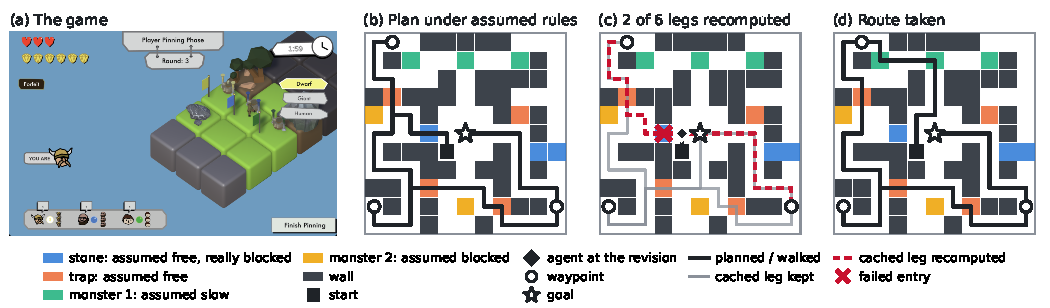
\includegraphics[width=0.75\textwidth]{fig_game_walkthrough.pdf}
\caption{(a) Dice Adventure, the game whose planning agent prompted this work. (b--d) Indexed repair on that game's $11\times11$ level layout, under the simulator's rules. An entry into a stone cell fails, the stone rule is committed as costlier, and only the 2 of 6 cached legs that list it are recomputed.}
\label{fig:walk}
\end{figure*}

\paragraph{The index.} The agent caches an optimal leg between every pair of remaining waypoints. A commit can make a cached leg wrong in two ways: a rule on its path was revised, or its path is untouched but a rule it \emph{avoided} became cheaper and another path now beats it. With each leg $\ell$ from $a$ to $b$ of cost $C_\ell$ the agent therefore stores one set of rules for each case:
\begin{itemize}
\item $\mathrm{val}(\ell)$, the \emph{direct support}: the types of the cells the leg enters. If none of these changes, the leg's cost is unchanged.
\item $\mathrm{blk}(\ell)$, the \emph{alternative support}: the types $k \notin \mathrm{val}(\ell)$ that have some cell $x$ with $d(a,x) + d(x,b) + \epsilon < C_\ell$, where $d$ is Manhattan distance and $\epsilon$ is the least amount by which an obstacle cell costs more than an open one.
\end{itemize}
The test for $\mathrm{blk}$ is a lower bound. A path from $a$ to $b$ through $x$ enters at least $d(a,x)+d(x,b)$ cells, each costing at least 1, and $x$ itself costs at least $\epsilon$ more. If even this bound is not below $C_\ell$, no price for rule $k$ can make a path through $x$ beat the leg, so $k$ need not be watched. When rule $k$ becomes costlier, the legs with $k \in \mathrm{val}$ are invalidated. When it becomes cheaper, the legs with $k \in \mathrm{val} \cup \mathrm{blk}$ are. Invalidated legs are recomputed, legs from the agent's current position are refreshed, and the ordering is solved again over the table. Everything else is kept (Figure~\ref{fig:walk}).

\begin{proposition}
Assume that under every committed model an open cell costs 1 to enter and an obstacle cell at least $1+\epsilon$, and that the table holds optimal legs under the committed model. After a commit that changes the cost of one or more rules, recomputing only the invalidated legs and re-solving the ordering gives a plan whose cost equals that of a plan computed from scratch under the new model.
\end{proposition}
\begin{proof}[Proof sketch]
Take a leg $\ell$ that is kept. No rule in $\mathrm{val}(\ell)$ changed, so its stored path still costs $C_\ell$. Suppose another path now costs less than $C_\ell$. Before the commit it cost at least $C_\ell$, so it became cheaper, so it enters a cell $x$ of some rule $k$ that became cheaper. By the bound above its new cost is at least $d(a,x)+d(x,b)+\epsilon$, which is therefore below $C_\ell$; hence $k \in \mathrm{blk}(\ell)$ or $k \in \mathrm{val}(\ell)$ and $\ell$ would have been invalidated. The argument is path by path, so it holds when one commit raises some rules and lowers others. Kept legs thus stay optimal, and the ordering uses exact costs.
\end{proof}
Here $\epsilon = 1/0.9 - 1$: no belief can price an obstacle cell below the expected attempts of a free one. The assumption is needed: if an obstacle could cost 1, an exhaustive search of $3\times3$ boards finds revisions the index misses; with the floor it finds none in 15.7 million, and an independent solver finds none in 10 million leg checks on random $4\times4$ and $5\times5$ boards whose commits mix increases, decreases and cell exceptions. The guarantee is of equal cost under the committed expected-cost model. It does not fix which of several equally cheap paths is kept, and it says nothing about realised cost. No saving is guaranteed \citep{nebel1995}: it depends on how many legs list the revised rule, and $\mathrm{blk}$ over-approximates.

\paragraph{Cell exceptions.} Proposition~1 covers rule commits. Walling off a single cell after eight consecutive failures there raises one cell's cost, so by the first step of the proof only the legs that enter it are recomputed. Withdrawing exceptions lowers costs that no rule entry covers; the table is then rebuilt.

\paragraph{Counterfactual probing.} The agent can test an uncertain rule before relying on it. For a rule $k$ in its plan's support and a nearby cell of that type, it compares the expected cost of its current plan with that of walking there, attempting once, and continuing with the best plan under each posterior. The index answers each such counterfactual query by recomputing only the legs that list $k$.

\section{Experiment}

\paragraph{Environment.} Maps are random wall segments plus, for each of $K{=}5$ obstacle types, line segments a path may cross or go around. Two types are nominally free, one slow, two blocked. Five waypoints and a goal are placed so that all are connected through open cells; obstacles are thus shortcuts and every agent can always finish. Attempt outcomes are a hash of (map, cell, attempt number), shared by all agents.

\paragraph{Violations.} All revising agents start with probability 0.7 on each rule's nominal value. Per map we construct, where the map allows it: \emph{none}; \emph{block} and \emph{slow}, in which a free rule that the initial plan uses is in fact blocked or slow; \emph{unlock}, in which a blocked rule in the initial plan's support is in fact free; and \emph{out of language}, in which a rule the plan uses is blocked on the left half of the map and free on the right, which no hypothesis can represent.

\paragraph{Agents.} \emph{No revision} plans with the nominal rules and walls off a single cell after eight consecutive failures. \emph{Revise + replan} updates beliefs and recomputes the whole table at every commit. \emph{Posterior sampling} \citep{osband2013} plans against a rule set sampled from the belief and resamples after every attempt. \emph{Generic probing} tests the rule with the highest information gain per unit distance until every belief is resolved. \emph{Indexed repair} is our mechanism; \emph{indexed repair + probing} adds counterfactual probing, and \emph{replan + probing} evaluates the same probes by full recomputation. An \emph{oracle} that knows the true rules gives the reference for regret. Revising agents drop all cell exceptions if the goal becomes unreachable.

\paragraph{Protocol.} Board sizes $15^2$, $31^2$ and $51^2$. After debugging on 30 development maps, the analysis plan and our predictions were written down with a hash of the code, and the final run used 300 different maps per size. We report mean paired differences with 10,000-resample bootstrap intervals over episodes and Holm-corrected Wilcoxon tests. Computation is counted in search-node expansions, which are deterministic, and we separate the initial plan, which all agents share, from work done afterwards. Analyses marked $\dagger$ were added after the planned ones.

\section{Results}

\begin{table*}[t]
\centering
\small
\begin{tabular}{@{}lccc@{}}
\toprule
 & $15\times15$ & $31\times31$ & $51\times51$ \\
\midrule
\multicolumn{4}{@{}l}{\emph{Relevant violations pooled (block, slow, unlock)}} \\
Episodes & 600 & 753 & 728 \\
Replanning work, indexed $/$ full & 0.56 & 0.66 & 0.67 \\
Actions, indexed $-$ full & 0 (identical) & 0 (identical) & 0 (identical) \\
Actions, probing $-$ no probing & $-1.0$ {\footnotesize[-1.4, -0.7]} & $-3.1$ {\footnotesize[-4.0, -2.2]} & $-8.2$ {\footnotesize[-10.0, -6.4]} \\
Actions, probing $-$ posterior sampling & $-4.2$ {\footnotesize[-5.1, -3.2]} & $-17.8$ {\footnotesize[-20.6, -15.3]} & $-29.1$ {\footnotesize[-33.7, -24.6]} \\
Actions, probing $-$ generic probing & $-31.3$ {\footnotesize[-32.5, -30.0]} & $-45.8$ {\footnotesize[-48.2, -43.5]} & $-54.7$ {\footnotesize[-58.7, -50.6]} \\
Probing work, indexed $/$ unindexed & 0.49 & 0.68 & 0.71 \\
\midrule
\multicolumn{4}{@{}l}{\emph{No violation}} \\
Actions, revising $-$ not revising & $+2.7$ {\footnotesize[2.1, 3.5]} & $+7.8$ {\footnotesize[6.4, 9.2]} & $+19.8$ {\footnotesize[16.9, 22.8]} \\
Actions, probing $-$ no probing & $-0.6$ {\footnotesize[-0.9, -0.3]} & $-0.9$ {\footnotesize[-1.8, -0.2]} & $-2.2$ {\footnotesize[-3.8, -0.6]} \\
\midrule
\multicolumn{4}{@{}l}{\emph{True rule outside the hypothesis space}} \\
Actions, probing $-$ no probing & $-0.8$ {\footnotesize[-1.8, 0.0]} & $+2.2$ {\footnotesize[-0.9, 5.5]} & $+6.6$ {\footnotesize[0.8, 12.7]} \\
\midrule
\multicolumn{4}{@{}l}{\emph{Index against ground truth (all conditions)}} \\
Repairs checked & 4,102 & 6,338 & 6,730 \\
Repaired plan $\neq$ fresh plan & 0 & 0 & 0 \\
Changed legs missed & 0 & 0 & 0 \\
Legs invalidated & 15\% & 31\% & 34\% \\
Legs that really changed & 10\% & 18\% & 19\% \\
\midrule
\multicolumn{4}{@{}l}{\emph{Added after the planned analysis}$^\dagger$} \\
Direct support only: non-optimal repairs; extra actions, mean (max) & 2.5\%; 0.04 (9) & 11.5\%; 0.22 (49) & 20.2\%; 0.95 (51) \\
Time, indexed $/$ full replanning without index & 0.65 & 0.70 & 0.69 \\
Leg-table search $/$ A* on all legs: index, LPA*, both & 0.31, 0.15, 0.14 & 0.47, 0.27, 0.23 & 0.48, 0.30, 0.24 \\
\bottomrule
\end{tabular}

\caption{Comparisons on 300 held-out maps per board size. Brackets are 95\% paired-bootstrap intervals over episodes; resampling maps instead widens them slightly and changes no sign. Negative favours the first-named agent. ``Work'' is search-node expansions and ``time'' is wall-clock, both after the initial plan. Rows marked $\dagger$ were not pre-specified.}
\label{tab:primary}
\end{table*}

\paragraph{Full replanning versus indexed repair.} Indexed repair took exactly the same actions as full replanning in every one of the 2,081 violation episodes and used 0.56, 0.66 and 0.67 of the replanning work at the three sizes (Table~\ref{tab:primary}). Checked against ground truth, the repaired plan matched a from-scratch plan in all 17,170 repairs and the index never failed to invalidate a leg whose cost had changed. It did invalidate more than necessary: 15--34\% of legs were flagged where 10--19\% had really changed. In single-process wall-clock time, against a replanner that builds no index, repair took 0.65, 0.70 and 0.69 of the time after the initial plan; building supports was 4--11\% of its planning time.

\paragraph{Direct support versus the full index.} A simpler tracker invalidates a leg only when a rule it uses changes. On the same maps it left a plan costlier than the optimum after 2.5\%, 11.5\% and 20.2\% of repairs, because a rule the plan avoided had become cheaper. It did 0.84, 0.74 and 0.71 of the indexed work. The behavioural price was small on average (0.04, 0.2 and 0.9 extra actions per episode) and up to 51 in the worst episode.

\paragraph{The index versus incremental search$^\dagger$.} LPA* \citep{koenig2004} reuses the inside of one search; the index decides which searches run at all. We replayed the same revision sequences on the leg table with LPA*, on every leg and on only the legs the index invalidates. \emph{Search effort:} as a fraction of the node expansions of A* on every leg, the index with A* needed 0.31, 0.47 and 0.48; LPA* on every leg 0.15, 0.27 and 0.30; LPA* on the indexed legs 0.14, 0.23 and 0.24. Incremental search thus saves more search than the index, and the index removes a further 11--18\% on top of it. All four methods agreed on every leg cost (63,397 checks). \emph{Wall-clock time} orders them differently. An optimised LPA* took 0.41, 0.61 and 0.67 of the A* time, against 0.32, 0.49 and 0.50 for the index with A*; adding the index to it saved 16--20\%. Between commits the index keeps 2--6\,KiB of state and LPA* 89--968. Counting the initial build, which costs LPA* 2.2--2.6 times as much, the index with A* was fastest over these short episodes (0.69--0.71 of the A* time; LPA* 1.17--1.35). \emph{Regime:} per commit, the index pays when under about half the cached legs change and costs about 4\% when nearly all do; 61\% of commits changed none.

\paragraph{Probing: fewer actions, far more computation.} Probing reduced actions relative to not probing by 1.0, 3.1 and 8.2 at the three sizes and beat generic probing and posterior sampling. But it did 24--34 times the planning work of indexed repair alone, and once computation is priced at even 0.001 actions per node expansion it loses to plain indexed repair at every size. When the true rule depended on location, which no hypothesis could represent, probing was worse, but only on the largest board; our other written predictions held. With no violation, the agent that never revised was best, by 2.7, 7.8 and 19.8 actions; when a rule it trusted was blocked it was by far the worst (regret 40, 104 and 213).

\paragraph{On the game's own levels$^\dagger$.} We ran the same agents on the four larger Dice Adventure level layouts, from each of the three character starts, with the game's five obstacle kinds given the simulator's rule values; the game's dice, health and teamwork are not modelled. Setting aside 12 of 48 combinations (9 where the violation made the goal unreachable, 3 where no rule fitted) left 1,800 episodes. Indexed repair again took the same actions as full replanning in every episode, at 0.78 of the replanning work under violations.

\paragraph{False abandonment versus late recognition$^\dagger$.} On these levels obstacles must sometimes be crossed, and in 19 episodes (1.1\%) every revising agent, with or without the index, stopped short of a goal that was reachable; the agent that never revises finished all of them. The traces show one cause: an obstacle with true success 0.3 stood on the only route and failed 9 to 13 times running, the belief that its rule was blocked passed 0.95, the rule was committed at infinite cost, and the plan cost became infinite. The truth was inside the hypothesis space; the error was to treat a 95\% belief as certain when the action was to give up. We then tested one safeguard: a commit that would make the goal unreachable is staged, the rule keeps a finite cost, and the agent gives up only when the belief passes 0.999. All 19 episodes then finished and the other 1,781 were unchanged. Since the safeguard was designed on these episodes, we ran it unchanged on 1,750 new maps that require obstacle crossings. Of 5,275 episodes with a reachable goal, the original agent abandoned 42 (0.8\%) and the safeguarded agent none (95\% upper bound 0.17\%), at 0.6 more actions on average. The cost is in recognising real impossibility: on 1,310 episodes with an unreachable goal it stopped after 97 actions on average, not 46. On a third map set a threshold of 0.99 still abandoned 9 of 5,197 reachable goals; tighter ones abandoned none but gave up later.

\section{Related Work}

\emph{Truth maintenance} \citep{doyle1979} retracts derived beliefs whose reasons fail, and its reasons can already include a belief being absent. The index applies this to cached legs and adds a cheap, sound test for that dependency on grids.

\emph{Plan repair and optimality monitoring.} RepairSHOP \citep{warfield2007} propagates changed conditions through a truth maintenance system over task nodes; HOTRiDE \citep{ayan2007} and SHOPFixer \citep{goldman2020} redo a part of the task tree; \citet{zaidins2025} show that the main algorithms solve formally different problems. All track state conditions and take the domain model as given. \citet{fritz2007} monitor conditions for a plan's continued optimality under a fixed action theory; our alternative support specialises that idea to rule hypotheses, with a geometric certificate.

\emph{Incremental search.} Lifelong Planning A* \citep{koenig2004}, D* Lite \citep{koenig2002} and dynamic shortest-path algorithms \citep{ramalingam1996} update one search after edge costs change and would handle every revision here. The index works a level above them, and the two compose.

\emph{Revising models and gathering information.} \citet{weber2011} and the systems named in the introduction revise action models after surprises and then replan. Our probing rule is metareasoning \citep{russell1991,lin2015} that approximates Bayes-adaptive planning \citep{guez2012}; \citet{tewari2026} derives a threshold policy for repairing, replanning or abandoning a plan under a fixed model.

\emph{Rollback for agent state.} ALAS \citep{chang2025} keeps dependency graphs for local compensation, ChronoMem \citep{su2026} versions agent memory and restores snapshots, and EvoCF \citep{chi2026} induces constraints from failures. The index restores nothing; it records the dependencies that selective rollback would need.

\section{Limitations}

The plan has two levels and the environment is a grid we built; nothing here shows the result carries to deep task hierarchies, and we did not compare against SHOPFixer or IPyHOPPER; the incremental-search comparison covers the leg table and one implementation. The layout is fully observed and rules are independent across types. The alternative support rests on a geometric bound that is specific to grids and loosens with board size. Other thresholds were set once and not swept. A pre-declared rerun with a more confident prior (0.9) left the repair result unchanged and shrank the probing gain to 0.3, 1.5 and 5.9 actions. The analyses marked $\dagger$ were chosen after seeing results. Finally, the first final-map run exposed a bug in our posterior-sampling baseline; we fixed it and reran.

\bibliography{refs}

\end{document}
